\chapter{RGB-D SLAM}\label{rgbd-slam}

 Range sensors have emerged as one of the most effective sensors to make robots autonomous. Unlike vision, range data makes the construction of a 3D model of the robot's environment straightforward and the Velodyne sensor, that combines 64 scanning lasers into one package, was key in mastering the DARPA Grand Challenge.  3D range data has become even more important in robotics with the advent of cheap (priced at a tenth than the cheapest 2D laser scanner) RGB-D (color image plus depth) cameras. Point cloud data allows fitting of lines using RANSAC, which can serve as features in EKF-based localization, but can also be used for improving odometry, loop-closure detection, and mapping. The goals of this chapter are
\begin{itemize}
\item introduce the Iterative Closest Point (ICP) algorithm
\item show how ICP can be improved by providing initial guesses via RANSAC
\item show how SIFT features can be used to improve point selection and loop-closure in ICP to achieve RGB-D mapping
\end{itemize}

\section{Converting range data into point cloud data}
Point cloud data can be thought of a 3D matrix that maps a certain volume in 3D space. Each cell in this matrix, also known as \emph{Voxel}\index{Voxel}, corresponds to whether there is an obstacle in this volume or not. Different intensity values could correspond to the uncertainty with which this space is to be known to be an obstacle. An efficient method to turn range information into such an uncertainty 3D map is described in \cite{curless96} and became known as \emph{Truncated Surface Distance Function} (TSDF)\index{Truncated Surface Distance Function (TSDF)}\index{TSDF}, commonly referred to as ``Point cloud''\index{Point cloud}.

\section{The Iterative Closest Point (ICP) algorithm}
The \emph{Iterative Closest Point} (ICP)\index{Iterative Closest Point}\index{ICP} algorithm was presented in the early 1990s for registration of 3D range data to CAD models of objects. A more in-depth overview of what is described here is given in \cite{rusinkiewicz01}. The key problem can be reduced to find the best transformation that minimizes the distance between two point clouds. This is the case when matching snapshots from a range sensor or matching a range image with a point cloud sampled from a 3D representation of an object.

In robotics, ICP found an application to match scans from 2D laser range scanners. For example, the transformation that minimizes the error between two consecutive snapshots of the environment is proportional to the motion of the robot. This is a hard problem as it is unclear, which points in the two consecutive snapshots are ``pairs", which of the points are outliers (due to noisy sensors), and which points need to be discarded as not all points overlap in both snapshots. Stitching a series of snapshots together theoretically allows to create a 2D map of the environment. This is difficult, however, as the error between every snapshots --- similar to odometry --- accumulates.   The ICP algorithm also works in 3D where it allows to infer the change in 6D pose of a camera and creation of 3D maps. In addition, ICP has proven useful for identifying objects from a database of 3D objects.

Before providing a solution to the mapping problem, we will focus on the ICP algorithm to match 2 consecutive frames. Variants of the ICP algorithm can be broken down into 6 consecutive steps:
\begin{enumerate}
\item Selection of points in one or both meshes or point clouds.
\item Matching/Pairing these points to samples in the other point cloud/mesh.
\item Weighting the corresponding pairs.
\item Rejecting certain pairs.
\item Assigning an error metric based on the point pairs.
\item Minimizing the error metric.
\item Point Selection
\end{enumerate}
Depending on the number of points generated by the range sensor, it might make sense to use only a few selected points to calculate the optimal transformation between two point clouds, and then test this transformation on all points. Depending on the source of the data, it also turns out that some points are more suitable than others as it is easier to identify matches for them. This is the case for RGB-D data, where SIFT features have been used successfully. This is also the case for planar objects with grooves, where sampling should ensure that angles of normal vectors of sampling points are broadly distributed. Which method to use is therefore strongly dependent on the kind of data being used and should be considered for each specific problem.

\subsection{Matching Points}
The key step in ICP is to match one point to its corresponding point.  For example, a laser scanner hits a certain point at a wall with its 67th ray. After the scanner has been moved by 10 cm, the closest hit on the wall to this point might have been by the 3rth ray of the laser. Here, it is actually very unlikely that the laser hits the exact same point on the wall twice, therefore introducing a non-zero error even for optimal pairing. Prominent methods are to find the closest point in the other point cloud or to find the intersection of the source points normal with the destination surface (for matching point clouds to meshes). More recently, SIFT has allowed to match points based on their visual appearance. Similarly to sorting through SIFT features, finding the closest matching point can be accelerated by representing the point cloud in a k-d tree.

\subsection{Weighting of Pairs}
As some pairs are better matches than others, weighting them in some smart way might drastically improve the quality of the resulting transformation. One approach is to give more weight to points that have smaller distances from each other. Another approach is to take into account the color of the point (in RGB-D images) or use the distance of their SIFT features (weighting pairs with low distances higher than pairs with high distances). Finally, expected noise can be used to weight pairings. For example, the estimates made by a laser scanner are much more faithful when taken orthogonally to a plane than when taken at a steep angle.

\subsection{Rejecting of Pairs}
A key problem in ICP are outliers either from sensor noise or simply from incomplete overlap between two consecutive range images. A prime approach in dealing with this problem is to reject pairings of which one of the points lies on a boundary of the point cloud as these points are likely to match with points in non-overlapping regions. As a function of the underlying data, it might also make sense to reject pairings with too high of a distance. This is a threshold-based equivalent to distance-based weighting as described above.

\subsection{Error Metric and Minimization Algorithm}
After points have been selected and matched, pairs have been weighted and rejected, the match between two point clouds needs to be expressed by a suitable error metric, which needs then to be minimized. A straightforward approach is to consider the sum of squared distances between each pair. This formulation can often be solved analytically. Let
\begin{eqnarray}
A=\{a_1,\ldots,a_n\}\\
B=\{b_1,\dots,b_n\}
\end{eqnarray}
be point clouds in $ \mathbb{R}^n$. The goal is now to find a vector $ t \in \mathbb{R}^n$ so that an error function $ \phi(A+t,B)$ is minimized. In 6D (translation and rotation), an equivalent notation can be found for a transformation (see forward kinematics). An error function for the squared distance is then given by
\begin{equation}
\phi(A+t,B)=\frac{1}{n}\sum_{a \in A}\|a+t-N_B(a+t)\|^2
\end{equation}
Here $ N_B(a+t)$ is a function that provides the nearest neighbor of $ a$ translated by $ b$ in $ B$.  A key problem now is that the actual value of $t$ affects the outcome of the pairing. What might look like a good match initially often turns out not be the final pairing. A simple numerical approach to this problem is to find $ t$ iteratively.

Initially $t=0$ and nearest neighbors/pairings are established. We can now calculate a $ \delta t$ that optimizes the least-square problem based on this matching using any solver available for the optimization problem (for a least-square solution $ \delta t$ can be obtained analytically by solving for the minimum of the polynomial by setting its derivative to zero). We can then shift all points in $ A$ by $ \delta t$ and start over. That is, we calculate new pairings and derive a new $ \delta t$.  We can continue to do this, until the cost function reaches a local minimum.

Instead of formulating the cost function as a ``point-to-point'' distance, a ``point-to-plane'' has become popular. Here, the cost function consist of the sum of squared distances from each source point to the plane that contains the destination point and is oriented perpendicular to the destination normal. This makes particularly sense when matching a point cloud to a mesh/CAD model of an object. In this case there are no analytical solutions to finding the optimal transformation, but any optimization method such a Levenberg-Marquardt can be used.

\section{RGB-D Mapping}
The ICP algorithm can be used to stitch consecutive range images together to create a 3D map of the environment \cite{henry2010rgb}. Together with RGB information, it is possible to create complete 3D walk throughs of an environment. An example of such a walk through using the method described in \cite{whelan2013robust} is shown in Figure \ref{fig:kintinous}.
A problem with ICP is that errors in each transformation propagate making maps created using this method as odd as maps created by simple odometry. Here, the SLAM algorithm can be used to correct previous errors once a loop closure is detected.


\begin{figure}
\centering
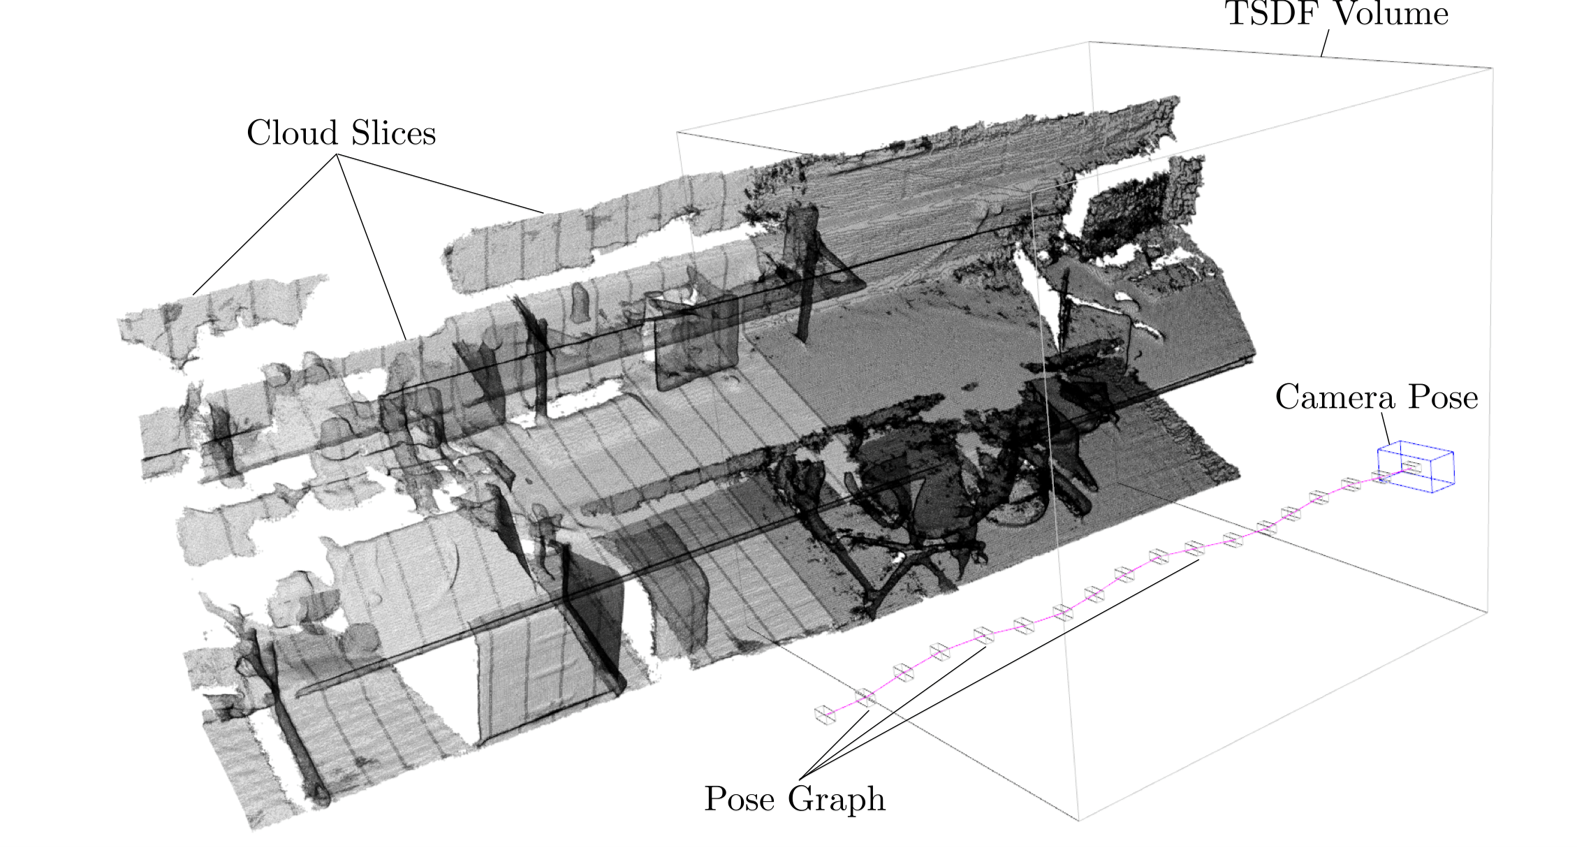
\includegraphics[width=\textwidth]{figs/kintinous}
\caption{Fused point cloud data from a walk trough of an office environment using ``Kintinious''. Picture courtesy of John Leonard.\label{fig:kintinous}}
\end{figure}

The intuition behind SLAM is to consider each transformation between consecutive snapshots as a spring with variable stiffness. Whenever the robot returns to a previously seen location, i.e., a loop-closure has been determined, additional constraints are introduced and the collection of snapshots connected by springs become a mesh. Everytime the robot then re-observes a transformation between any of the snapshots, it can ``stiffen'' the spring connecting the two. As all of the snapshots are connected, this new constraints propagates through the network and literally pull each snapshots in place.

RGB-D Mapping uses a variant of ICP that is enhanced by SIFT features for point selection and matching. Maps are build incrementally. SIFT features, and their spatial relationship, are used for detecting loop closures. Once a loop closure is detected, an additional constraint is added to the pose graph and a SLAM-like optimization algorithm corrects the pose of all previous observations.

As ICP only works when both point clouds are already closely aligned, which might not be the case for a fast moving robot with a relatively noisy sensor (the XBox Kinect has an error of 3cm for a few meters of range vs. millimeters in laser range scanners), RGB-D Mapping uses RANSAC to find an initial transformation. Here, RANSAC works as for line fitting: it keeps guessing possible transformations for 3 pairs of SIFT feature points and then counts the number of inliers when matching the two point clouds, one of which being transformed using the random guess.
